\section{Analysis}

\begin{tabular}{lrr}
\toprule
   Alias Name &           \# &          \% \\
\midrule
    \verb|ls| &  \num{83782} &   \num{3.8} \\
    \verb|ll| &  \num{62465} &  \num{2.83} \\
  \verb|grep| &  \num{44479} &  \num{2.02} \\
    \verb|la| &  \num{43760} &  \num{1.99} \\
     \verb|l| &  \num{39539} &  \num{1.79} \\
\bottomrule
\end{tabular}
\hspace{0.3cm}
\begin{tabular}{lrr}
    \toprule
           Command &            \# &           \% \\
    \midrule
        \verb|git| &  \num{327786} &  \num{12.93} \\
         \verb|ls| &  \num{260156} &  \num{10.27} \\
         \verb|cd| &  \num{166632} &   \num{6.58} \\
       \verb|grep| &   \num{89598} &   \num{3.54} \\
        \verb|vim| &   \num{46545} &   \num{1.84} \\
    \bottomrule
\end{tabular}
\hspace{0.3cm}
\begin{tabular}{lrr}
    \toprule
                Argument &            \# &          \% \\
    \midrule
     \verb|--color=auto| &  \num{153931} &  \num{4.24} \\
               \verb|-i| &   \num{70640} &  \num{1.95} \\
               \verb|-a| &   \num{42910} &  \num{1.18} \\
               \verb|-l| &   \num{39519} &  \num{1.09} \\
               \verb|-v| &   \num{35295} &  \num{0.97} \\
    \bottomrule
\end{tabular}



\Cref{tab:top-summary} shows the most common alias names, commands, and arguments appearing in alias definitions.
The most common alias name we found is \texttt{ls}, appearing a total number of \num{83782} times, which is \per{3.8} of all alias definitions.
Note that this is \texttt{ls} as an \emph{alias name}, a redefinition of the \texttt{ls} \emph{command}, which appears \num{260156} times (\per{10.27}).
This is a bit less often than \texttt{git}, the most common command, which appears in \num{327786} aliases (\per{12.93}).
The most common argument, across all commands, is \texttt{--color=auto}, appearing \num{153931} times (\per{4.24})

\newcommand{\numx}[1]{{\small (\num{#1})}}
\begin{table}
    \caption{Top two commands with top arguments and aliases}
    \label{tab:command-summary}
    \begin{tabular}{@{}lrll@{}}
        \toprule
                    &           \% &            Arguments &                                                                 Aliases (\%) \\
        \midrule
         \verb|git| &   \num{5.85} &        \verb|status| &                              \verb|gs| \numx{54.27}, \verb|gst| \numx{19.19} \\
                    &   \num{3.48} &              \verb|| &                                \verb|g| \numx{75.71}, \verb|gti| \numx{5.74} \\
                    &   \num{3.20} &      \verb|checkout| &      \verb|gco| \numx{50.52}, \verb|gc| \numx{13.87}, \verb|gch| \numx{7.56} \\
                    &   \num{3.18} &          \verb|push| &      \verb|gp| \numx{46.73}, \verb|gps| \numx{9.23}, \verb|push| \numx{7.56} \\
                    &   \num{3.16} &          \verb|diff| &                                                       \verb|gd| \numx{79.89} \\
                    &   \num{2.86} &          \verb|pull| &      \verb|gpl| \numx{18.30}, \verb|gl| \numx{16.59}, \verb|gp| \numx{15.07} \\
                    &   \num{2.78} &        \verb|branch| &                               \verb|gb| \numx{73.54}, \verb|gbr| \numx{6.57} \\
                    &   \num{2.71} &           \verb|add| &                                                       \verb|ga| \numx{80.96} \\
                    &   \num{2.00} &        \verb|commit| &                               \verb|gc| \numx{63.16}, \verb|gci| \numx{5.33} \\
                    &   \num{1.96} &     \verb|commit -m| &       \verb|gcm| \numx{31.29}, \verb|gc| \numx{25.18}, \verb|gm| \numx{7.97} \\
        \midrule
          \verb|ls| &  \num{14.45} &  \verb|--color=auto| &                                                       \verb|ls| \numx{99.04} \\
                    &   \num{8.63} &            \verb|-A| &                                                       \verb|la| \numx{97.61} \\
                    &   \num{7.80} &           \verb|-CF| &                                                        \verb|l| \numx{98.75} \\
                    &   \num{6.78} &          \verb|-alF| &                                                       \verb|ll| \numx{97.49} \\
                    &   \num{5.46} &            \verb|-l| &                                 \verb|ll| \numx{78.83}, \verb|l| \numx{7.91} \\
                    &   \num{3.75} &              \verb|| &                                \verb|l| \numx{27.90}, \verb|sl| \numx{21.45} \\
                    &   \num{2.88} &            \verb|-G| &                                                       \verb|ls| \numx{96.47} \\
                    &   \num{2.74} &           \verb|-la| &      \verb|ll| \numx{38.42}, \verb|la| \numx{26.87}, \verb|lla| \numx{12.63} \\
                    &   \num{2.67} &            \verb|-a| &                                                       \verb|la| \numx{76.94} \\
                    &   \num{1.92} &           \verb|-al| &         \verb|ll| \numx{49.69}, \verb|la| \numx{12.23}, \verb|l| \numx{8.49} \\
        \bottomrule
    \end{tabular}
\end{table}



\newcommand{\rot}[1]{\makebox[1em][l]{\rotatebox{45}{#1}}}

\newcommand{\full}{$\CIRCLE$}
\newcommand{\half}{$\LEFTcircle$}
\newcommand{\empt}{$\Circle$}

\newcommand{\hist}[1]{\includegraphics[height=1em, trim=1em 1em 1em 1em, clip]{compression/#1.pdf}}

\newcommand*{\pie}[1]{\begin{tikzpicture}[scale=0.15]%
    \draw (0,0) circle (1);
    \fill[fill opacity=1,fill=black] (0,0) -- (90:1) arc (90:90-#1*3.6:1) -- cycle;
    \end{tikzpicture}}

\begin{table*}
    \caption{Common commands broken down by alias use cases}
    \label{tab:use-cases}
    \begin{tabular}{llrlllllccc}
        & & \# & &\rot{Default Arguments} & \rot{Autocorrect} & \rot{Chaining} & \rot{Safety} & \rot{Bookmarks} & & Compression \\
        \midrule
        \multicolumn{2}{l}{Version Control} \\
            & \texttt{git}                                  & \num{629593} & & & & \pie{5.84} & &             & & \hist{git} \\
            & \texttt{hg}                                   & \num{29363} &  & & &	\pie{4.66}  & &             & & \hist{hg} \\
        \midrule
        \multicolumn{2}{l}{System Tools} \\
            & \texttt{ls}                                   & \num{384186} & & \pie{27.11} & & \pie{2.29} &             &             & & \hist{ls} \\
            & \texttt{cd}                                   & \num{229522} & & & & \pie{4.79} &             & \pie{63.37} & & \hist{cd} \\
            & \texttt{grep}*                                & \num{223629} &  & \pie{63.02} & & \pie{24.29} &       & \pie{1.51} & & \hist{grep} \\
            & \texttt{echo}                                 & \num{53934} &  & \pie{1.14} & & \pie{31.27} &             &  \pie{7.54} & & \hist{echo} \\
            & \texttt{xargs}                                & \num{44927} &  & & & \pie{35.27} &             &             & & \hist{xargs} \\
            & \texttt{ssh}                                  & \num{36574} &  & \pie{4.54} & & \pie{3.46} &             & \pie{64.39} & & \hist{ssh} \\
            & \texttt{rm}                                   & \num{44209} &  & \pie{48.29} & & \pie{13.02} & \pie{56.53} & \pie{22.68} & & \hist{rm} \\
            & \texttt{dir}                                  & \num{31069} &  & \pie{99.55} & & &             &             & & \hist{dir} \\
            & \texttt{cp}                                   & \num{27472} &  & \pie{76.35} & & \pie{4.72} & \pie{70.61} & \pie{12.62} & & \hist{cp} \\
            & \texttt{mv}                                   & \num{22689} &  & \pie{83.03} & & \pie{3.12} & \pie{79.21} & \pie{5.56}  & & \hist{mv} \\
            & \texttt{sort}                                 & \num{22391} &  & & & \pie{87.04} &             &             & & \hist{sort} \\
            & \texttt{head}                                 & \num{17530} &  & & & \pie{78.32} &             & \pie{1.04}  & & \hist{head} \\
            & \texttt{cat}                                  & \num{17425} &  & & & \pie{15.16} & \pie{1.81}  & \pie{42.48} & & \hist{cat} \\
            & \texttt{port}                                 & \num{11228} &  & & &\pie{3.79}  & \pie{96.75} &             & & \hist{port} \\
        \midrule
        \multicolumn{2}{l}{Package Managers} \\
            & \texttt{zypper}                           & \num{66295} & & & & & \pie{93.36} &           & & \hist{zypper} \\
            & \texttt{pacman}                           & \num{46821} & & \pie{2.81} & & \pie{1.22} & \pie{69.21} &           & & \hist{pacman} \\
            & \texttt{mvn}                              & \num{36683} & & & & \pie{1.09} &             &           & & \hist{mvn} \\
            & \texttt{yaourt}                           & \num{34577} & & & & &             &           & & \hist{yaourt} \\
            & \texttt{apt}*                         & \num{74991} & &  \pie{9.8}&   & \pie{10.16} &  \pie{45.0}           &           & & \hist{apt} \\
            & \texttt{brew}                             & \num{27060} & & & & \pie{39.49} &             &           & & \hist{brew} \\
        \midrule
        \multicolumn{2}{l}{Text Editors}  \\
            & \texttt{mate}                             & \num{61832} & & & & &             & \pie{95.77} & & \hist{mate} \\
            & \texttt{vim}                              & \num{0} &     & \pie{3.28} & & \pie{3.28} & \pie{5.1}   & \pie{44.02} & & \hist{vim} \\
            & \texttt{nvim}                             & \num{0} &     & & & \pie{1.19} & \pie{1.72}  & \pie{17.38} & & \hist{nvim} \\
            & \texttt{emacs}                            & \num{10299} & & \pie{18.44} & \pie{10.75} & \pie{1.16} & \pie{2.19}  & \pie{10.83} & & \hist{emacs} \\
        \midrule
        \multicolumn{2}{l}{Developer Tools} \\
            & \texttt{wp}                               & \num{66434} & & & & &             &             & & \hist{wp} \\
            & \texttt{zeus}                             & \num{52570} & & & & \pie{12.09} &             & \pie{23.91} & & \hist{zeus} \\
            & \texttt{php}                              & \num{44486} & & & & \pie{7.06}&             & \pie{6.9}   & & \hist{php} \\
        \midrule
        \multicolumn{2}{l}{Infrastructure} \\
            & \texttt{docker}*  & \num{73706} & & & & \pie{3.86} & \pie{2.63} & \pie{7.6} & & \hist{docker} \\
            & \texttt{kubectl}*                                      & \num{39781} & & & & & & & & \hist{kubectl} \\
            & \texttt{vagrant}                                                  & \num{8953} &  & & & \pie{11.17} & & & & \hist{vagrant} \\
        \midrule
        \multicolumn{2}{l}{Other} \\
            & \texttt{ffmpeg}                             & \num{606} & & \pie{14.69} & & \pie{8.75} &            & \pie{30.2} & & \hist{ffmpeg} \\
            & \texttt{beep}                               & \num{85} &  & \pie{4.71} & & \pie{50.59} & \pie{4.71} &            & & \hist{beep} \\
    \end{tabular}
\end{table*}
 % TODO: update

Looking at each part of an alias definition in isolation can only get us so far, as arguments only gain meaning in conjunction with commands and alias names can be identical between users, referring to the same command/argument combination, or indeed can overlap, meaning the same alias name is used differently by different users.
\Cref{tab:command-summary} gives a more informative view for the top two commands, \texttt{git} and \texttt{ls}, showing us the top arguments given with each and the most common alias names by which the command/argument combinations are referred to.
Here we can already identify some of the different customization practices involving aliases.
Looking at \texttt{ls}, we find that aliases are used
to redefine the command with a default argument (\verb|alias ls="ls --color=auto"|);
to shorten a common invocation (\verb|alias ll="ls -alF"|);
and to correct a spelling mistake (\verb|alias sl=ls|).
We also notice that in the case of \texttt{git}, most aliases are used for shortening \texttt{git} subcommand invocations (e.g. \verb|alias gd="git diff"|).

To capture the range of patterns and use cases for which aliases are defined, we applied inductive coding methods on a selected cross-section of the dataset.
We looked at 1381 alias definitions derived in a similar way as \Cref{tab:command-summary}, i.e. the most common aliases for the most common arguments for the most common commands.
In addition, we took a random sample of 200 alias definitions that each occur only once in the dataset to represent the long tail.
Coding was then performed independently by two authors, who labelled each alias definition in the cross-section with descriptive tags, taking the semantics of the commands as much as possible into account.\footnote{The website \url{https://explainshell.com} has been an indispensable resource.}
Inductive coding is an iterative process between theoretical sampling and comparing data within emerging themes \cite{thomas:06,dey:03}.
After a first iteration, the coders compared their labels, consolidating different naming conventions.
In consecutive iterations, the coders identified ways of formalizing the emerged categories, i.e. constructing automated mechanisms for classifying alias definitions as belonging into a certain category or not.
The discussion of the formalizations additionally served to establish a better shared understanding.
Ultimately, the coders reached a saturation point at which further coding and analysis did not lead to further insights.

We could identify \TODO customization practices involving aliases:

\TODO

\Cref{tab:use-cases} breaks down the customization practices by command, presenting a selection of commands with a quantitative overview about the kinds of aliases each command is commonly used in.

We will now discuss each of the \TODO customization practices in more detail.

%We explore the range of patterns and use cases for which Shell aliases are defined.
First, we provide an overview and quantify common structures in our dataset regarding alias uses, commands, and arguments.
Based on the initial exploration, we then present both quantitative and qualitative results from different aspects of alias usage.

The single most common alias definition in our dataset is
\begin{verbatim}
alias '${1+"$@"}'="$@"
\end{verbatim}
appearing \num{78265} times, which is \per{1.64} of all alias definitions.
This curious jumble of symbols derives from a portability hack for \texttt{zsh}.\footnote{\url{https://unix.stackexchange.com/a/191836}}

More familiar results can be seen in \Cref{tab:top-summary}, which shows the most common alias names, commands, and arguments appearing in alias definitions.
The most common alias name we found is \texttt{ls}, appearing a total number of \num{124515} times, which is \per{2.61} of all alias definitions.
Note that this is \texttt{ls} as an \emph{alias name}, a redefinition of the \texttt{ls} \emph{command}, which appears \num{378097} times (\per{7.12}).
This is about half as often as \texttt{git}, the most common command, which appears in \num{626185} aliases (\per{11.79}).
The most common argument, across all commands, is \texttt{--color=auto}, appearing \num{268171} times (\per{3.6})

\begin{table*}
    \caption{Top alias names, commands and arguments}
    \label{tab:top-summary}
    \begin{tabular}{lrr}
        \toprule
                 Alias Name &            \# &          \% \\
        \midrule
                  \verb|ls| &  \num{124515} &  \num{2.61} \\
                  \verb|ll| &   \num{89254} &  \num{1.87} \\
         \verb|'${1+"$@"}'| &   \num{78265} &  \num{1.64} \\
                \verb|grep| &   \num{63392} &  \num{1.33} \\
                  \verb|la| &   \num{62039} &  \num{1.30} \\
        \bottomrule
    \end{tabular}
    \hspace{0.1cm}
    \begin{tabular}{lrr}
        \toprule
               Command &            \# &           \% \\
        \midrule
            \verb|git| &  \num{626185} &  \num{11.79} \\
             \verb|ls| &  \num{378097} &   \num{7.12} \\
             \verb|cd| &  \num{229522} &   \num{4.32} \\
           \verb|grep| &  \num{128045} &   \num{2.41} \\
           \verb|"$@"| &   \num{78276} &   \num{1.47} \\
        \bottomrule
    \end{tabular}
    \hspace{0.1cm}
    \begin{tabular}{lrr}
        \toprule
                    Argument &            \# &          \% \\
        \midrule
         \verb|--color=auto| &  \num{268171} &  \num{3.60} \\
                   \verb|-i| &  \num{109094} &  \num{1.47} \\
                   \verb|-v| &   \num{70424} &  \num{0.95} \\
                   \verb|-l| &   \num{63302} &  \num{0.85} \\
                   \verb|-a| &   \num{62023} &  \num{0.83} \\
        \bottomrule
    \end{tabular}        
\end{table*}

Looking at each part of an alias definition in isolation can only get us so far, as arguments only gain meaning in conjunction with commands and alias names potentially vary widely.
\Cref{tab:command-summary} gives a more informative view, centered around some common commands, showing us the top arguments given with each command and the most common alias names by which the command/argument combinations are referred to.
Here we can see \TODO

\begin{table*}
    \caption{Common commands and their top arguments and aliases}
    \label{tab:command-summary}
    \begin{tabular}{lrll}
        \toprule
             Command &           \% &                 Arguments &                                                                                 Aliases (\%) \\
        \midrule
          \verb|git| &   \num{3.75} &             \verb|status| &                                  \verb|gs| (\num{51.57}), \verb|gst| (\num{24.17}) \\
                     &   \num{2.42} &           \verb|checkout| & \verb|gco| (\num{51.17}), \verb|gc| (\num{10.04}), \verb|letcat| (\num{9.18}) \\
                     &   \num{2.33} &               \verb|push| &    \verb|gp| (\num{49.12}), \verb|rulz| (\num{9.53}), \verb|gps| (\num{7.15}) \\
                     &   \num{2.31} &                   \verb|| &                                                                  \verb|g| (\num{78.87}) \\
                     &   \num{2.18} &               \verb|pull| &    \verb|gl| (\num{25.32}), \verb|gpl| (\num{13.29}), \verb|gp| (\num{11.53}) \\
                     &   \num{2.11} &               \verb|diff| &                                                                 \verb|gd| (\num{83.21}) \\
                     &   \num{2.05} &                \verb|add| &                              \verb|ga| (\num{73.01}), \verb|chicken| (\num{10.85}) \\
                     &   \num{2.01} &             \verb|branch| &                                   \verb|gb| (\num{74.88}), \verb|gbr| (\num{8.26}) \\
                     &   \num{1.59} &          \verb|commit -m| & \verb|gcm| (\num{21.67}), \verb|gcmsg| (\num{19.59}), \verb|gc| (\num{18.18}) \\
                     &   \num{1.20} &             \verb|commit| &                                                                 \verb|gc| (\num{65.51}) \\
        \midrule
           \verb|ls| &  \num{13.15} &       \verb|--color=auto| &                                                                 \verb|ls| (\num{99.09}) \\
                     &   \num{9.12} &                 \verb|-A| &                                                                 \verb|la| (\num{98.27}) \\
                     &   \num{8.57} &                \verb|-CF| &                                                                  \verb|l| (\num{98.94}) \\
                     &   \num{6.69} &                 \verb|-l| &                                                                 \verb|ll| (\num{82.64}) \\
                     &   \num{6.63} &               \verb|-alF| &                                                                 \verb|ll| (\num{97.89}) \\
                     &   \num{3.65} &                   \verb|| &      \verb|l| (\num{21.38}), \verb|sl| (\num{16.99}), \verb|iz| (\num{12.24}) \\
                     &   \num{3.06} &                 \verb|-G| &                                                                 \verb|ls| (\num{97.46}) \\
                     &   \num{2.43} &                \verb|-la| &      \verb|ll| (\num{32.80}), \verb|la| (\num{22.61}), \verb|l| (\num{12.71}) \\
                     &   \num{2.01} &                 \verb|-a| &                                                                 \verb|la| (\num{74.80}) \\
                     &   \num{1.77} &               \verb|-lah| &     \verb|l| (\num{32.64}), \verb|lsa| (\num{31.61}), \verb|ll| (\num{19.01}) \\
        \midrule
         \verb|grep| &  \num{36.12} &       \verb|--color=auto| &                                                               \verb|grep| (\num{99.29}) \\
                     &  \num{12.50} &                   \verb|| &   \verb|G| (\num{22.27}), \verb|hgrep| (\num{10.98}), \verb|rrg| (\num{7.22}) \\
                     &   \num{4.42} &            \verb|--color| &                                                               \verb|grep| (\num{97.00}) \\
                     &   \num{1.68} &                 \verb|-i| &        \verb|grep| (\num{6.88}), \verb|G| (\num{5.86}), \verb|g| (\num{5.86}) \\
                     &   \num{1.52} & \verb|--color=never '^d'| &                                                                \verb|lsd| (\num{98.45}) \\
        \bottomrule
    \end{tabular}
\end{table*}

One drawback of this presentation is that there are obviously many different ways of how arguments to a command can be combined.
For most programs, the order of arguments does not matter and often there are multiple ways to specify the same argument.
\Cref{tab:command-summary} obscures the long tail of argument variations.
In order to get more insight into how aliases are used, we will now look at the dataset with certain use cases in mind. 


\subsection{Default Arguments}

One common use case of using aliases was to define commands with default arguments.
More specifically, we refer to an alias as defining default arguments when the alias name is the same as the command name, and in the alias definition, the command specifies at least one further argument.
This phenomenon can be already observed in Tables \ref{tab:top-summary} and \ref{tab:command-summary} for commands \verb|ls| and \verb|grep| (e.g., \verb|alias ls='ls -G'| or \verb|alias grep='grep -i'|).
Overall, aliases defining default arguments make up a sizable amount of \num{502801} (\per{10.5}) of all alias definitions. 
Interestingly, a majority of these aliases, \num{278370} (\per{55.4}), deal with enabling color in commands (e.g., \verb|--color=auto|, \verb|--color=always|).
The top 3 aliases (or 6 depending on whether you would want to count basic synonyms separately) make up more than \per{95} of the \per{55.4}: \verb|dir|/\verb|vdir| (\per{21.7}), \verb|ls| (\per{26.5}), and \verb|grep|/\verb|fgrep|/\verb|egrep| (\per{49.3}).
Since aliases defining color as their default argument would disproportionally skew any relative measure from other data we observed, we exclude them when reporting summary statistics for the remainder of this section.

To a much lesser extent, we saw two other patterns emerging: (1) enabling interactivity in commands, and (2) enabling human-readable and verbose outputs.
We also saw safety and interactivity as part of a broader trend beyond just aliases for default arguments and report more results on this pattern in Section \ref{sec:safety}.
To quickly summarize the extent within default arguments: \num{64497} aliases define interactivity arguments (or \per{28.7} of overall default argument aliases without color options).
Default arguments that enable human-readable and verbose outputs were present in \num{35080} aliases (or \per{15.6} of overall default argument aliases without color options).
%Table \ref{tab:default-arguments-overview} provides an overview of the most common aliases defining default arguments (when removing color options).



\subsection{Autocorrect}

Another trend we observed in our exploration was that of aliases introducing manually defined autocorrect rules for misspelled commands (e.g., \verb|gti| instead of \verb|git|).
While it is easy for the human eye to determine instances of these typographical errors, it is not as straightforward to formalize all different cases.
We opt for a conservative measure (potentially underestimating the true extent of the phenomenon) in which autocorrecting aliases are defined as alias names with the same string length as their associated commands with a distance measure above an empirically determined threshold.
We surveyed and experimented with different distance measures~\cite{navarro:01} and decided on using the Damerau-Levenshtein measure~\cite{damerau:64}.
It is a robust algorithm that in addition to tracking the number of insertions, deletions, and substitutions between two strings, also captures the transposition of two characters, a common occurrence in misspelled commands.  
%We use the Jaro similarity metric~\cite{jaro:89}, as it is a widespread distance measure that was introduced to capture typographical errors.
%Querying alias names with the same length as command names, but differ in their content (i.e., they do not define default arguments) returns \num{518500} (\per{10.86}) results.
We query alias names with the same length as command names, but that differ in their content (i.e., they do not define default arguments), apply the Damerau-Levenshtein algorithm, and normalize the result.
Normalized distances are a float in the range of 0 and 1, where 0 entails there are no differences between the two strings and 1 means the distance is as far as it can be (corresponding to the length of the longer string in the original score).
We compute the results, order by normalized score, and empirically determine $\frac{1}{3}$ (roughly corresponding to \per{33} difference between autocorrecting alias name and command name) to be considered a conservative threshold to determine misspellings.
This results in \num{63875} (\per{1.3}) total aliases that serve as autocorrect rules.
Table \ref{tab:autocorrect} provides an overview of interesting autocorrecting aliases with different distance measures.

\begin{table}[]
	\caption{A curated selection from autocorrecting aliases highlighting a variety of use cases together with their normalized Damerau-Levenshtein distance}
		\label{tab:autocorrect}
	\begin{tabular}{@{}lllr@{}}
		\toprule
		Alias Name & Command & Reason & Score \\ 
		\midrule
		\verb|grpe|, \verb|sduo| & \verb|grep|, \verb|sudo| & Transposition & \num{0.25} \\
		\verb|pluralize| & \verb|pluralise| & Localized Spelling & 0.11 \\
		\verb|Jupyter| & \verb|jupyter| & Case-sensitivity & 0.14 \\
		\verb|ungzip| & \verb|gunzip| & Mismatched casing & 0.33 \\ 
		\begin{tabular}[c]{@{}l@{}}\Verb|docker-build|,\\ \verb|mysql.server|\end{tabular} & \begin{tabular}[c]{@{}l@{}}\verb|docker_build|, \\ \verb|mysql-server|\end{tabular} & Punctuation & 0.08 \\
		\bottomrule
	\end{tabular}
\end{table}



\subsection{Compression}

\begin{figure}
    \centering
    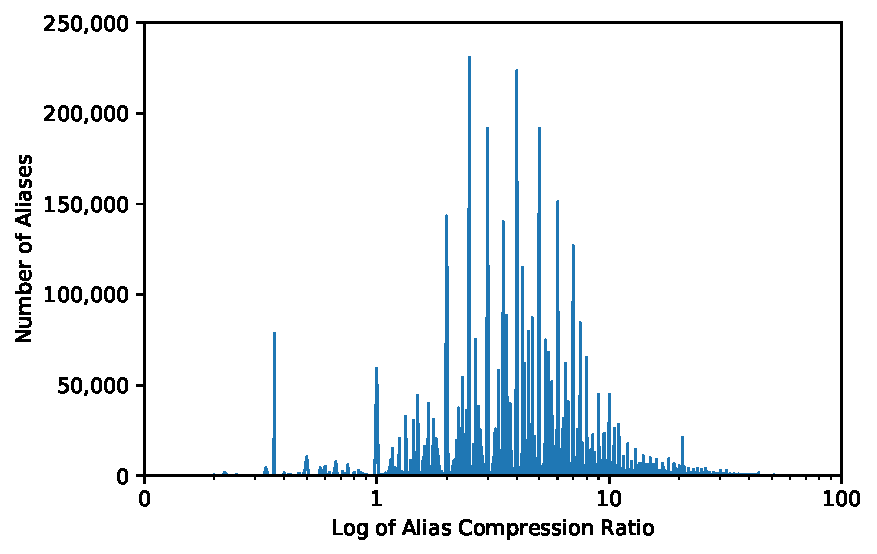
\includegraphics[width=\columnwidth]{compression_dist.pdf}
    \caption{Distribution of alias compression ratios}
    \label{fig:compression}
\end{figure}

One use of aliases is to simplify complex expressions by giving them short, memorable names.
The average length of an alias name is \num{4.43} characters, whereas the average length of an alias value is \num{21.15} characters.
If we divide the length of an alias value by the length of the alias name, we get the \emph{compression ratio} of the alias.
For example, the definition
\begin{CVerbatim}
alias gs='git status'
\end{CVerbatim}
has a compression ratio of 5.
\Cref{fig:compression} shows the distribution of compression ratios over all aliases in the dataset.
The median compression ratio is 4.2, meaning half of all alias values are at least four times as long as their alias names.
A compression ratio less than 1 indicates an alias name that is longer than the value it aliases.
\Cref{tab:use-cases} gives at-a-glance compression distributions for aliases using common commands in first position.
The mini-histograms are log-log scaled; red lines mark the compression ratio 1.

There are \num{157542} aliases (\per{3.3}) with names longer than their values.%
\footnote{The curious spike at 0.36 in \cref{fig:compression} is the \texttt{zsh} portability hack described earlier.
It makes up \per{49.68} of long alias names.}
Among them, we found many descriptive names, like
\begin{itemize}
    \item \verb|git-last-commit-message|
    \item \verb|docker_list_all_containers|
    \item \verb|generate_random_password|
\end{itemize}
and similar wordy descriptions of simple command invocations.
Additionally, we found compatibility aliases (like \texttt{md5sum} for \texttt{md5}) and many humorous definitions (like \texttt{kthxbai} for \texttt{halt} or \texttt{please} for \texttt{sudo}).

The two longest alias names we found are from joke definitions.
The first is \num{1772} characters long and is comprised of the letter `f' repeated \num{1053} times, followed by the letter `u' repeated \num{719} times.
It is an alias for the \texttt{cat} command with a similarly named file as an argument.
The second longest alias name is a Swedish compound word of \num{131} characters,\footnote{Translating, roughly, to northwestern-glacier-artillery-flight-thrust-simulator-plant-equipment-maintenance-follow-up-systems-discussion-posts-preparation-works.} aliasing the \texttt{ls} command.

On the other end of the spectrum, the highest compression ratio in any alias definition comes from an alias named \texttt{BEEP}, which invokes the Linux \texttt{beep} utility 9 times in succession, with a combined \num{4471} arguments.
When executed, it appears to play Daft Punk's 2001 instrumental single \emph{Aerodynamic}.


\subsection{Chaining} 

In addition to the number of arguments, another source of complexity in aliases (i.e. value length) is command composition or chaining.
\num{351060} aliases (\per{7.36}) are composed of more than one command.
The most popular way to combine commands is with a pipe (\verb!|!), used by \per{35.2} of multi-command aliases, closely followed by logical conjunction (\verb|&&|), used by \per{29.75}, and simple chaining (\verb|;|), used by \per{28.4}.
Other operators (\verb|&|, \verb!||!, \verb!|&!) appear in only \per{6.65} of multi-command aliases.
\Cref{tab:operators} shows the top commands in 2nd, 3rd and 4th position of a command chain, for each possible preceding operator.

\begin{table}[h]
	\caption{Top commands following operators}
	\label{tab:operators}
	\begin{tabular}{ll|l|l}    
		\toprule
		& 2nd position & 3rd position & 4th position \\
		\midrule
		\verb!|! & \verb|grep| {\small (\num{34.17})} & \verb|grep| {\small (\num{14.56})} & \verb|xargs| {\small (\num{19.25})} \\     
		& \verb|sort| {\small (\num{11.1})} & \verb|head| {\small (\num{12.37})}& \verb|head| {\small (\num{17.52})}\\ 
		& \verb|xargs| {\small (\num{6.4})} & \verb|sort| {\small (\num{8.81})} & \verb|grep| {\small (\num{11.35})}\\ 
		\midrule
		\verb!&&! & \verb|git| {\small (\num{16.73})} & \verb|git| {\small (\num{16.26})} & \verb|git| {\small (\num{12.47})} \\ 
		& \verb|killall| {\small (\num{8.81})} & \verb|aur| {\small (\num{16.05})} & \verb|date| {\small (\num{8.25})}\\ 
		& \verb|abs| {\small (\num{8.57})} & \verb|startpost| {\small (\num{4.51})} & \verb|brew| {\small (\num{6.44})} \\ 
		\midrule
		\verb!;! & \verb|git| {\small (\num{8.53})} & \verb|zeus| {\small (\num{10.18})} & \verb|brew| {\small (\num{9.29})}\\ 
		& \verb|echo| {\small (\num{6.63})}& \verb|git| {\small (\num{10.06})}  & \verb|echo| {\small (\num{8.15})} \\ 
		&  \verb|cd| {\small (\num{4.84})} & \verb|cd| {\small (\num{5.74})} &  \verb|git| {\small (\num{6.49})}\\ 
		\midrule
		\verb!||! & \verb|alias| {\small (\num{46.37})} & \verb|echo| {\small (\num{18.86})} & \verb|echo| {\small (\num{20.67})} \\ 
		& \verb|tmux| {\small (\num{19.26})} & \verb|tmux| {\small (\num{8.32})}  &  \verb|cd| {\small (\num{20.11})} \\ 
		& \verb|true| {\small (\num{4.56})} &  \verb|umount| {\small (\num{7.41})} & \verb|true| {\small (\num{13.41})}\\ 
		\midrule
		\verb!&! & \verb|disown| {\small (\num{15.12})} & \verb|disown| {\small (\num{16.92})} & \verb|amp| {\small (\num{7.51})} \\
		& \verb|/dev/null| {\small (\num{13.65})} & \verb|!| {\small (\num{6.95})} & \verb|disown| {\small (\num{7.51})} \\
		& \verb|~/X| {\small (\num{5.49})} & \verb|exit| {\small (\num{4.51})} & \verb|exit| {\small (\num{6.36})} \\    
		\midrule
		\verb!|&! & \verb|less| {\small (\num{71.53})} & \verb|grep| {\small (\num{61.54})} & \verb|tee| {\small (\num{100.0})} \\
		& \verb|tee| {\small (\num{11.81})}  & \verb|less| {\small (\num{15.38})} &  \\
		& \verb|grep| {\small (\num{9.03})} & \verb|color| {\small (\num{7.69})} &  \\
		\midrule
	\end{tabular}
\end{table}

% I think this table might be misleading, because it ranks commands by relative occurrence with operators, rather then normalizing with overall command occurrence. That's probably why git dominates &&

The most interesting operator is certainly the pipe (\verb!|!), since it creates an interface between two otherwise separate programs.
\Cref{fig:flow} shows a flow diagram of the top 200 pipelines with three commands that make up at least \per{10} of one participating command's usage.

\begin{figure*}[h]
	\centering    
	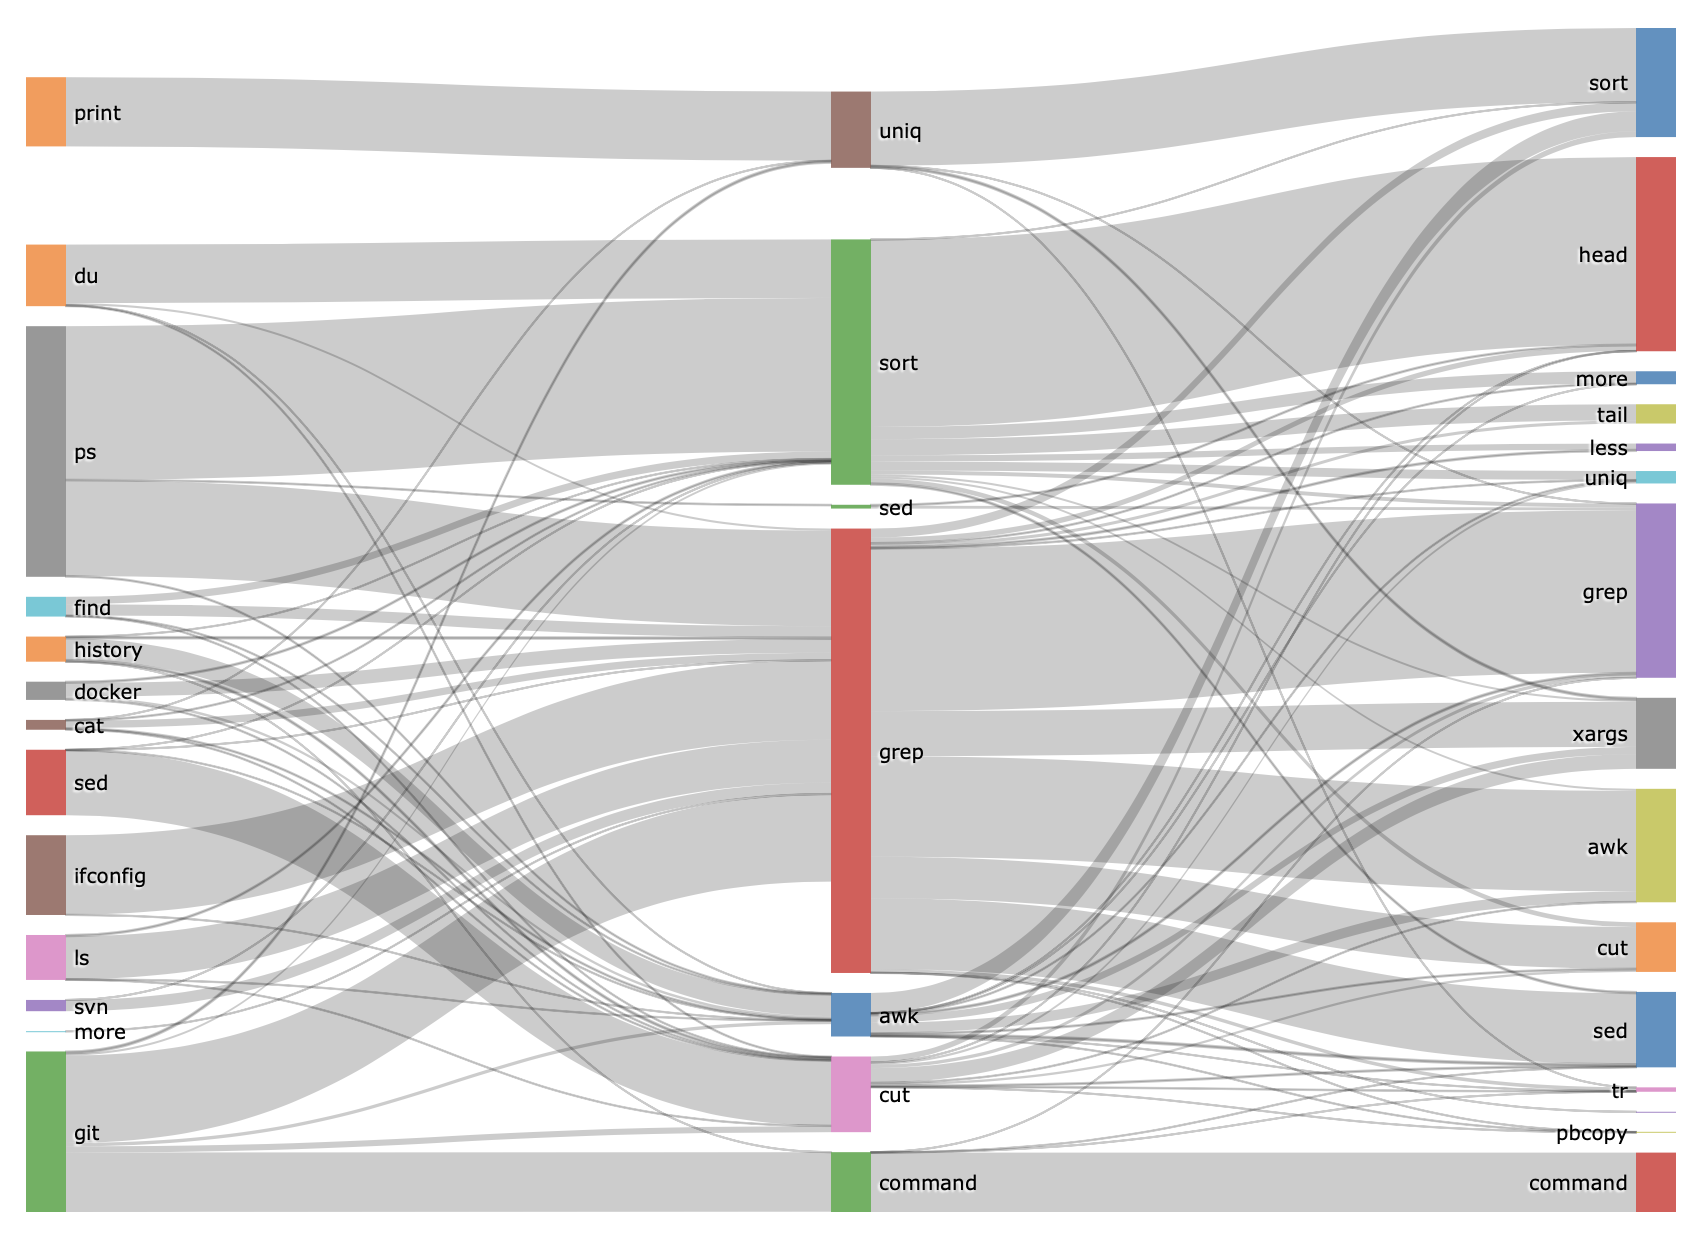
\includegraphics[width=0.78\linewidth]{flow.png}
	\caption{Flow diagram for top 3-command pipelines}
	\label{fig:flow}
\end{figure*}


\subsection{Safety and Interactive Mode}
\label{sec:safety}

The \texttt{sudo} command allows the user to execute another command with superuser privileges.
In our dataset, we found \num{336298} commands (\per{6.3}) prefixed with \texttt{sudo}, used in \num{305637} alias definitions (\per{6.4}).
The top 10 commands used with \texttt{sudo} are given in \cref{tab:sudo-commands}.

Remarkably, 8 out of the top 10 \texttt{sudo}-prefixed commands are related to package managers:
\texttt{zypper} (openSUSE); \texttt{pacman}, \texttt{abs} and \texttt{aur} (Arch Linux); \verb|apt-get| and \verb|$apt-pref| (Debian, Ubuntu); \texttt{yum} (RPM); and \texttt{dnf} (Fedora).
Even more remarkable: all of these commands are used with \texttt{sudo} the majority of the time they are used.

Some users even go so far as to redefine certain commands to always be executed with \texttt{sudo}, mostly system utilities like \texttt{reboot} or \texttt{shutdown}, but also (again) package managers like \texttt{pacman} and \texttt{apt}.
However, on the whole this practice appears to be relatively rare (see \cref{tab:sudo-redefine}).

\begin{table}
    \caption{Top 10 commands used with \texttt{sudo}.}
    \label{tab:sudo-commands}
    \begin{tabular}{lrrl}
      \toprule
      Command & \multicolumn{1}{c}{\#} & \multicolumn{1}{c}{With \texttt{sudo}} & Description \\
      \midrule  
      \verb|zypper|    & \num{66295} & \num{61891} (\per{93.36})  & package manager\\
      \verb|pacman|    & \num{46821} & \num{32407} (\per{69.21})  & package manager \\
      \verb|apt-get|   & \num{34075} & \num{28323} (\per{83.12})  & package manager \\
      \verb|$apt_pref| & \num{20245} & \num{20245} (\per{100.00}) & package manager \\
      \verb|yum|       & \num{23940} & \num{12843} (\per{53.65})  & package manager \\
      \verb|dnf|       & \num{24469} & \num{12697} (\per{51.89})  & package manager \\
      \verb|port|      & \num{11228} & \num{10863} (\per{96.75})  & networking utility \\
      \verb|abs|       &  \num{9909} &  \num{9905} (\per{99.96})  & package manager \\
      \verb|aur|       &  \num{8837} &  \num{8795} (\per{99.52})  & package manager \\
      \verb|systemctl| & \num{13942} &  \num{7018} (\per{50.34})  & system utility \\
      \bottomrule
    \end{tabular}
\end{table}

\begin{table}
    \caption{Top 10 commands redefined to always use \texttt{sudo}}
    \label{tab:sudo-redefine}
    \begin{tabular}{llrl}
        \toprule
        Alias Name & Alias Value & \# & Description \\
        \midrule
        \verb|pacman|    & \verb|sudo pacman|    & 901 & package manager \\
        \verb|reboot|    & \verb|sudo reboot|    & 809 & system utility \\
        \verb|shutdown|  & \verb|sudo shutdown|  & 499 & system utility \\
        \verb|apt-get|   & \verb|sudo apt-get|   & 455 & package manager \\
        \verb|docker|    & \verb|sudo docker|    & 345 & container platform \\
        \verb|halt|      & \verb|sudo halt|      & 230 & system utility \\
        \verb|apt|       & \verb|sudo apt|       & 228 & package manager \\
        \verb|systemctl| & \verb|sudo systemctl| & 184 & system utility \\
        \verb|htop|      & \verb|sudo htop|      & 180 & system utility \\
        \verb|poweroff|  & \verb|sudo poweroff|  & 169 & system utility \\
        \bottomrule
    \end{tabular}
\end{table}

On the other end of the safety spectrum, some users default to running the file system commands \texttt{rm}, \texttt{cp}, and \texttt{mv} in interactive mode, which prompts before performing potentially destructive actions.
Taking into account variations between systems and different ways to enable interactive mode, \per{44.37} of alias definitions invoking \texttt{rm} are redefinitions of \texttt{rm} enabling interactive mode by default.
Those numbers are even higher for \texttt{cp} and \texttt{mv}, where \per{68.27} and \per{77.62} of uses are redefinitions, respectively (see \cref{tab:interactive}).

\begin{table}
    \caption{Commands commonly used in interactive mode}
    \label{tab:interactive}
    \begin{tabular}{lrrr}
        \toprule
        Command & \multicolumn{1}{c}{\#} & \multicolumn{1}{c}{With \texttt{-i}} & \multicolumn{1}{c}{Redefined With \texttt{-i}} \\
        \midrule
        rm & \num{44209} & \num{20300} (\per{45.92}) & \num{19617} (\per{44.37}) \\
        cp & \num{27472} & \num{18994} (\per{69.14}) & \num{18755} (\per{68.27}) \\
        mv & \num{22689} & \num{17842} (\per{78.64}) & \num{17611} (\per{77.62}) \\
        \bottomrule
    \end{tabular}
\end{table}






\subsection{Bookmarks}

We define a \emph{bookmark} to be an alias containing an argument that references some specific local or remote location, e.g. a file path, domain or IP address.
For instance, 
\begin{CVerbatim}
alias dl="cd ~/Downloads"
\end{CVerbatim}
and
\begin{CVerbatim}
alias starwars="telnet towel.blinkenlights.nl"
\end{CVerbatim}
are both bookmark aliases.

To find such bookmarks in our dataset, we searched for arguments that are locations, which we take to be any of the following:
\begin{itemize}
    \item An IPv4 address, matched by the liberal regular expression \verb|[0-9]+.[0-9]+.[0-9]+.[0-9]+|
    \item A string containing one of the known top-level domains\footnote{From \url{http://data.iana.org/TLD/tlds-alpha-by-domain.txt} (retrieved January 14, 2020)} preceded by a dot (\verb|.|) and followed by a slash (\verb|/|), colon (\verb|:|) or the end of the string.
    \item A string containing a forward slash (\verb|/|), indicating a path.
\end{itemize}
To avoid false positives, we sampled the top 300 search results according to the above criteria and determined some exclusion patterns.
For instance, \texttt{/dev/null} is not a location for our purposes.
Neither is \texttt{origin/master}, and thus 
\begin{CVerbatim}
alias gm="git merge origin/master"
\end{CVerbatim}
does not count as a bookmark.

By our definition, \num{282358} aliases (\per{12.1}) are bookmarks.
Of these, only \num{22381} are remote bookmarks (containing URLs or IP addresses).
Bookmarks are used predominantly for file system navigation, and the \texttt{cd} command is featured heavily in bookmark aliases.
Most other uses seem to be development related, like starting services such as web servers or databases with pre-defined locations, or outputting log files, as in 
\begin{CVerbatim}
alias onoz="cat /var/log/errors.log"
\end{CVerbatim}
or opening frequently edited files, as in the most common bookmark overall, which is for editing the shell configuration itself:
\begin{CVerbatim}
alias ohmyzsh="mate ~/.oh-my-zsh"
\end{CVerbatim}
\Cref{tab:bookmarks} shows the top 5 local and remote bookmarks.

\begin{table}
    \caption{Top 5 local and remote locations in bookmarks}
    \label{tab:bookmarks}
    \begin{tabular}{lr}
        \toprule
        Location & \# \\        
        \midrule
        \verb|~/.zshrc| & \num{27710} \\
        \verb|~/.oh-my-zsh| & \num{19068} \\
        \verb|../..| & \num{7520} \\
        \verb|../../..| & \num{5577} \\
        \verb|~/.bashrc| & \num{3763} \\
        \midrule
        \verb|myip.opendns.com| & \num{2373} \\
        \verb|@resolver1.opendns.com| & \num{2354} \\
        \verb|nyancat.dakko.us| & \num{537} \\        
        \verb|8.8.8.8| & \num{465} \\
        \verb|127.0.0.1| & \num{384} \\
        \bottomrule
    \end{tabular}
\end{table}

% for potential related work (including method), google 'usability smells'
% e.g. https://www.sciencedirect.com/science/article/pii/S1071581916301215
%      https://link.springer.com/chapter/10.1007/978-3-662-44811-3_13